%% BioMed_Central_Tex_Template_v1.05
%%                                      %
%  bmc_article.tex            ver: 1.05 %
%                                       %


%%%%%%%%%%%%%%%%%%%%%%%%%%%%%%%%%%%%%%%%%
%%                                     %%
%%  LaTeX template for BioMed Central  %%
%%     journal article submissions     %%
%%                                     %%
%%         <27 January 2006>           %%
%%                                     %%
%%                                     %%
%% Uses:                               %%
%% cite.sty, url.sty, bmc_article.cls  %%
%% ifthen.sty. multicol.sty		       %%
%%									   %%
%%                                     %%
%%%%%%%%%%%%%%%%%%%%%%%%%%%%%%%%%%%%%%%%%


%%%%%%%%%%%%%%%%%%%%%%%%%%%%%%%%%%%%%%%%%%%%%%%%%%%%%%%%%%%%%%%%%%%%%
%%                                                                 %%	
%% For instructions on how to fill out this Tex template           %%
%% document please refer to Readme.pdf and the instructions for    %%
%% authors page on the biomed central website                      %%
%% http://www.biomedcentral.com/info/authors/                      %%
%%                                                                 %%
%% Please do not use \input{...} to include other tex files.       %%
%% Submit your LaTeX manuscript as one .tex document.              %%
%%                                                                 %%
%% All additional figures and files should be attached             %%
%% separately and not embedded in the \TeX\ document itself.       %%
%%                                                                 %%
%% BioMed Central currently use the MikTex distribution of         %%
%% TeX for Windows) of TeX and LaTeX.  This is available from      %%
%% http://www.miktex.org                                           %%
%%                                                                 %%
%%%%%%%%%%%%%%%%%%%%%%%%%%%%%%%%%%%%%%%%%%%%%%%%%%%%%%%%%%%%%%%%%%%%%


\NeedsTeXFormat{LaTeX2e}[1995/12/01]
\documentclass[10pt]{bmc_article}    



% Load packages
\usepackage{cite} % Make references as [1-4], not [1,2,3,4]
\usepackage{url}  % Formatting web addresses  
\usepackage{ifthen}  % Conditional 
\usepackage{multicol}   %Columns
\usepackage[utf8]{inputenc} %unicode support
\usepackage{verbatim}
\usepackage{graphicx}
%\usepackage[applemac]{inputenc} %applemac support if unicode package fails
%\usepackage[latin1]{inputenc} %UNIX support if unicode package fails
\urlstyle{rm}
 
 
%%%%%%%%%%%%%%%%%%%%%%%%%%%%%%%%%%%%%%%%%%%%%%%%%	
%%                                             %%
%%  If you wish to display your graphics for   %%
%%  your own use using includegraphic or       %%
%%  includegraphics, then comment out the      %%
%%  following two lines of code.               %%   
%%  NB: These line *must* be included when     %%
%%  submitting to BMC.                         %% 
%%  All figure files must be submitted as      %%
%%  separate graphics through the BMC          %%
%%  submission process, not included in the    %% 
%%  submitted article.                         %% 
%%                                             %%
%%%%%%%%%%%%%%%%%%%%%%%%%%%%%%%%%%%%%%%%%%%%%%%%%                     
%\def\includegraphic{}
%\def\includegraphics{}

\setlength{\topmargin}{0.0cm}
\setlength{\textheight}{21.5cm}
\setlength{\oddsidemargin}{0cm} 
\setlength{\textwidth}{16.5cm}
\setlength{\columnsep}{0.6cm}

\newboolean{publ}

%%%%%%%%%%%%%%%%%%%%%%%%%%%%%%%%%%%%%%%%%%%%%%%%%%
%%                                              %%
%% You may change the following style settings  %%
%% Should you wish to format your article       %%
%% in a publication style for printing out and  %%
%% sharing with colleagues, but ensure that     %%
%% before submitting to BMC that the style is   %%
%% returned to the Review style setting.        %%
%%                                              %%
%%%%%%%%%%%%%%%%%%%%%%%%%%%%%%%%%%%%%%%%%%%%%%%%%%
 

%Review style settings
%\newenvironment{bmcformat}{\begin{raggedright}\baselineskip20pt\sloppy\setboolean{publ}{false}}{\end{raggedright}\baselineskip20pt\sloppy}

%Publication style settings
\newenvironment{bmcformat}{\fussy\setboolean{publ}{true}}{\fussy}



% Begin ...
\begin{document}
\begin{bmcformat}


%%%%%%%%%%%%%%%%%%%%%%%%%%%%%%%%%%%%%%%%%%%%%%
%%                                          %%
%% Enter the title of your article here     %%
%%                                          %%
%%%%%%%%%%%%%%%%%%%%%%%%%%%%%%%%%%%%%%%%%%%%%%

\title{Faunus: An Object Oriented Framework for Molecular Si\-mu\-la\-tion}
 
%%%%%%%%%%%%%%%%%%%%%%%%%%%%%%%%%%%%%%%%%%%%%%
%%                                          %%
%% Enter the authors here                   %%
%%                                          %%
%% Ensure \and is entered between all but   %%
%% the last two authors. This will be       %%
%% replaced by a comma in the final article %%
%%                                          %%
%% Ensure there are no trailing spaces at   %% 
%% the ends of the lines                    %%     	
%%                                          %%
%%%%%%%%%%%%%%%%%%%%%%%%%%%%%%%%%%%%%%%%%%%%%%


\author{
Mikael Lund\correspondingauthor$^{1}$%
       \email{Mikael Lund\correspondingauthor - mikael.lund@uochb.cas.cz}%
\and
Martin Trulsson$^{2}$
\and
Bj\"orn Persson$^{2}$
      }
      
%%%%%%%%%%%%%%%%%%%%%%%%%%%%%%%%%%%%%%%%%%%%%%
%%                                          %%
%% Enter the authors' addresses here        %%
%%                                          %%
%%%%%%%%%%%%%%%%%%%%%%%%%%%%%%%%%%%%%%%%%%%%%%

\address{%
    \iid(1) Institute of Organic Chemistry and Biochemistry, The Academy of Sciences of the Czech Republic, Flemingovo nam.2, CZ-16610 Prague 6, Czech Republic.
     \iid(2) Department of Theoretical Chemistry,
     University of Lund, P.O.B 124 SE-22100 Lund, Sweden.
}%

\maketitle

%%%%%%%%%%%%%%%%%%%%%%%%%%%%%%%%%%%%%%%%%%%%%%
%%                                          %%
%% The Abstract begins here                 %%
%%                                          %%
%% The Section headings here are those for  %%
%% a Research article submitted to a        %%
%% BMC-Series journal.                      %%  
%%                                          %%
%% If your article is not of this type,     %%
%% then refer to the Instructions for       %%
%% authors on http://www.biomedcentral.com  %%
%% and change the section headings          %%
%% accordingly.                             %%   
%%                                          %%
%%%%%%%%%%%%%%%%%%%%%%%%%%%%%%%%%%%%%%%%%%%%%%


\begin{abstract}
        % Do not use inserted blank lines (ie \\) until main body of text.
        \paragraph*{Background:} We present a C++ class library for Monte Carlo simulation of molecular systems, including proteins in solution. The design is generic and highly modular, enabling multiple developers to easily implement additional features. The statistical mechanical methods are documented by extensive use of code comments that -- subsequently -- is collected to automatically build a web-based manual.
        \paragraph*{Results:} We show how an object oriented design can be used to create an intuitively appealing coding framework for molecular simulation. This is exemplified in a \emph{minimalistic} C++ program that can calculate protein protonation states. We further discuss performance issues related to high level coding abstraction.

        \paragraph*{Conclusions:} C++ and the Standard Template Library (STL) provide a high-performance platform for generic molecular modelling. Automatic generation of code documentation from inline comments has proven particularly useful in that no seperate manual needs to be maintained.
\end{abstract}



\ifthenelse{\boolean{publ}}{\begin{multicols}{2}}{}




%%%%%%%%%%%%%%%%%%%%%%%%%%%%%%%%%%%%%%%%%%%%%%
%%                                          %%
%% The Main Body begins here                %%
%%                                          %%
%% The Section headings here are those for  %%
%% a Research article submitted to a        %%
%% BMC-Series journal.                      %%  
%%                                          %%
%% If your article is not of this type,     %%
%% then refer to the instructions for       %%
%% authors on:                              %%
%% http://www.biomedcentral.com/info/authors%%
%% and change the section headings          %%
%% accordingly.                             %% 
%%                                          %%
%% See the Results and Discussion section   %%
%% for details on how to create sub-sections%%
%%                                          %%
%% use \cite{...} to cite references        %%
%%  \cite{koon} and                         %%
%%  \cite{oreg,khar,zvai,xjon,schn,pond}    %%
%%  \nocite{smith,marg,hunn,advi,koha,mouse}%%
%%                                          %%
%%%%%%%%%%%%%%%%%%%%%%%%%%%%%%%%%%%%%%%%%%%%%%




%%%%%%%%%%%%%%%%
%% Background %%
%%
\section*{Background}
Molecular simulation has become a standard tool for investigating molecular systems such as proteins, polymer solutions, lamellar phases etc.
It is safe to say that for biological applications Molecular Dynamics (MD) is by far the most abundant method as it provides both static and dynamic properties of the system.
Metropolis Monte Carlo (MC) simulation~\cite{metropolis:53}, on the other hand, is less utilized and only few software packages exists\cite{Kamberaj:2001fk,carlsson:01,Jie-Hu:2006lr}.
One advantage of MC is that it allows ``unphysical'' particle moves, enabling very efficient sampling of the configurational space\cite{frenkel}. The tradeoff for this freedom to move particle is the loss of all dynamic information and, in addition, MC programs tend to become less general.
However, if one is interested in equilibrium properties only -- binding constants, free energy changes, pKa values etc. -- MC simulation may be a good option.

Using a standard, pre-compiled software package should require no prior knowledge of programming and as such can be a fast and practical approach for solving a specific scientific problem. On the other hand, the underlying physical theory is somewhat hidden and there is always a risk that the application is regarded as a ``black box'' producing numbers. It becomes even worse if new features are to be implemented.
The alternative is for researchers to create their own programs. This approach of course requires some programming skills and writing an advanced simulation program from scratch may be an overwhelming -- and likely error prone -- task.
Instead the programmer may resort to existing libraries, thus approaching the ``black box'' situation described above. However, the abstraction level will typically be lower which has several advantages that allows the researcher to
(i) be able to quickly develop a working program,
(ii) have a high level of control, and
(iii) experience high performance due a minimalistic design.

In this text we present a C++~\cite{stroustrup:97} framework or class library that can be used to quickly build customized MC simulation programs.

 %Text for this section.\cite{koon,oreg,khar,zvai,xjon,schn,pond,smith,marg,hunn,advi,koha,mouse}


%%%%%%%%%%%%%%%%%%
%
\section*{Implementation}
\subsection*{Object Oriented Design}
The object oriented capabilities of C++ have enabled us to create a suite of classes with an intuitive interface.
For example, the handling of particles -- a key undertaking of all classical simulations -- is provided by a class hierarchy:
\begin{verbatim}
class point {
public:
  double x,y,z;
  double dist(point &);
  ...
};
class particle {
public:
  double charge, radius;
  ...
};
\end{verbatim}
The Standard Template Library (STL) is subsequently used to construct a vector of particles, \verb"vector<particle>", that allows for easy access and manipulation.
For instance, \verb"p[i].radius" will return the size of the $i$'th particle.

\subsection*{Polymorphic Classes -- Virtual Functions}
One of the unique features of C++ is \emph{polymorph classes} that allows for very generic and intuitively appealing code.
To demonstrate this, we now outline the design of our framework for handling the simulation container -- see Figure~\ref{fig:container}.
Basically, the end programmer will want to select among different geometries -- a box, sphere, cylinder etc.
For each geometry we need functions that can calculate the volume, generate a random point and decide whether a given point falls within the boundaries.
We now construct a polymorph class, \verb"container", that contains the unimplemented \emph{virtual functions}.
Derived classes -- \verb"box", \verb"cylinder" etc. -- then implement specialized versions of the functions and the \verb"container" class hence acts as an interface to the various geometries.
This means that we can construct functions that accept any geometry derived from the \verb"container" class.
For example:
\begin{verbatim}
double concentration(container &c)
{ return N / c.volume(); }
\end{verbatim}.
Due to a large overhead, virtual functions may, however, negatively impact performance and are generally avoided in critical, inner loops.

\subsection*{Performance Aspects}
\subsubsection*{Function Inlining via Templates}
The most computationally demanding step in most molecular simulations is the evaluation of configurational energies.
Hence the applied pair potential must be highly optimized and preferably inlined in all inner loops.
This is accomplished by passing a pair potential \emph{class} as a template parameter that will create a local instance inside the inner loop template,
\begin{verbatim}
class coulomb {
  float energy(particle &a, particle &b)
  {
    return a.charge*b.charge/a.dist(b);
  }
};

template<class T_pairpot>
class innerloop {
  T_pairpot pair;
  float sum( vector<particle> &p ) {
    for (i=0; i<N-1; i++)
      for (j=i+1; j<N; j++) 
        u=u+pair.energy(p[i], p[j]);
    ...
};
\end{verbatim}
This so-called Expression Template technique~\cite{veldhuizen:95} enables the programmer to arbitrarily invoke various pair potential functions, re-cycling the inner loop implementation,
\begin{verbatim}
innerloop<coulomb> elec;
innerloop<lennardjones> lj;
elec.sum(p);
...
\end{verbatim}

\subsubsection*{Passing arguments as references}
In C++ argument passing is done by creating a new copy of the object. Working with large, aggregate structures such as particle vectors, this will negatively impact performance. To circumvent this we pass all complex objects as references, for example: \verb"void function(someclass &)".

\subsubsection*{Minimize memory comsumption}
Computer simulations of classical mechanical systems are usually not memory intensive and by minimizing the memory requirements there is a good chance that the executing code will stay in the local cache. In this regard C++ templates are a concern since code will be generated for each template type. We therefore stride to avoid extensive use of multiple template types -- for example it would seem silly to instantiate both a \verb"float" and a \verb"double" version of a template class.

\subsubsection*{Parallization}
In systems that equilibrate fast, Monte Carlo simulations can be linearly parallelized using the ``embarrasingly simple technique'' -- that is start several independent runs with different random seeds, combining the results afterwards.
Tightly coupled parallization is incorporated in parts of the code by threading the energy evaluation into two processes: before and after a trial move.
For systems with particles in the order of hundreds, this scales well on dual-core computers, whereas the overhead becomes unacceptable for small systems. To enable threading, the approprite compiler flag for OpenMP~\cite{openmp:98} must be set. The GNU, Intel and IBM C++ compilers all support OpenMP.

\subsection*{Code Documentation}
We provide a class library and as such need to describe both what the classes do as well as how to use them. This can be conveniently achieved using a code documentation system -- here we have chosen \verb"Doxygen"~\cite{doxygen} since (i) the documentation appears as normal code comments and (ii) the output is highly configurable, allowing LaTeX equations to be inserted etc.
For example, commenting a class like this,
\begin{verbatim}
/*!
 * \brief n'th degree Legendre polynomium
 * \author M. Lund
 * \date Canberra 2005-2006
 * Example\n
 * \code
 * legendre l(10);
 * l.eval(1.3);
 * cout << l.p[3]
 * \endcode
 */
class legendre { ... }
\end{verbatim}
will cause \verb"Doxygen" to recognize the individual keywords and include them in the manual (HTML, PDF etc).
Another very useful feature of Doxygen is the ability to generate a graphical view of the class hierachy. This enables the end programmer to visually see how a class is constructed as shown in Figure 1.



 
%%%%%%%%%%%%%%%%%%%%%%%%%%%%
%% Results and Discussion %%
%%
\section*{Results and Discussion}

\subsection*{General Features}
The class library provides simulation routines for ions, macromolecules and chains in solutions with a strong focus on electrostatic interactions using the primitive model of electrolytes~\cite{hill:86} where the solvent is treated as a structureless dielectric continuum. It is, however, completely possible to expand the library to other systems, include explicit solvent etc. The routines have been developed over several years in connection with a number of scientific investigations, including proteins in solution~\cite{lund:05}.
As of writing, the code library contains general classes for studying the following,
\begin{itemize}
\item Explicit treatment of ions, including ion-ion correlation effects.
\item Macromolecules -- Proteins, flexible chains, charged surfaces.
\item Proton titration of molecules.
\item Particle distribution functions and other statistical mechanical averages.
\item Popular file format are supported: PQR, Gromacs (GRO/XTC), Povray~\cite{povray}, XYZ.
\end{itemize}
An example of protein ionization will be presented later in the text.
We stress that the project is under ongoing development and encourage interested users and developers to contribute.

\subsubsection*{``Trajectory'' Output}
Molecular Dynamics simulation packages often save the time propagated particle trajectory to disk which is then subsequently analyzed.
In order to adopt this strategy we include an export routine that can dump the simulated particle configurations to a compressed Gromacs XTC file~\cite{gromacs}.
This (large) file can be analyzed using the extensive set of tools provided in the Gromacs package, or visualized using VMD~\cite{vmd}, for example.
As an example of the latter, we have simulated lysozyme interacting the a fab-H fragment and, using VMD, plotted the spatial mass center distribution as shown in Figure~\ref{fig:}


%    \subsubsection*{This is a sub-sub-heading}
   %   Sub-sub-sub-headings are made with the \textsl{\\subsubsection} command. \pb
 %     pb at end of lines ensures correct paragraph spacing.\pb
%	  Text for this sub-sub-section \ldots



\subsection*{An example}
Figure 2 shows a small code example for simulating the ionization state of a protein in a salt solution at various pH. Experimentally this corresponds to a standard potentiometric titration experiment where the net-charge is measured as a function of pH~\cite{tanford:72}. We will not go through all lines in the code as the comments should be more or less self-explanatory. The overall program structure is
\begin{enumerate}
\item Set up the simulation cell (line 13)
\item Add protein(s) and ions (line 21-28)
\item Main loop with salt- and proton moves (line 35)
\item Print results incl. Povray output (line 50-52)
\end{enumerate}
For simplicity we have left out the equilibration step but in this particular case it does not matter too much since the system equilibrates fast and the initial configurations will influence the overall statistics only to a minor extent.
Results and comparisons with experimental data for such calculations can be found in a recent article published by Lund \emph{et al.}~\cite{lund:07}.
Coordinates from any given configuration can be exported to various formats, including povray as shown in Figure 3.
Particles in the systems can be clustered into groups and derived classes and hence, there is a general group class (line 26), a class for macromolecules (line 19), chains etc. Note that we have also incorporated a general polymorphic class for markov moves and data analysis so that all derived classes have a common interface. For example, both the salt move (line 29) and titration class (line 30) will store information about energy changes, if the move was a success etc. Data and analysis about each type of move is automatically shown by calling the respective information functions (line 50).

%\subsection*{Another results sub-heading}
%    Text for this sub-section \ldots

%\subsection*{Yet another results sub-heading}
%    Text for this sub-section.  More results \ldots

%%%%%%%%%%%%%%%%%%%%%%
\section*{Conclusions}

\section*{Availability and requirements}
\textsl{Project name:} faunus\\
\textsl{Project home page:} http://faunus.sourceforge.net\\
\textsl{Operating systems:} MacOS X, Linux, UNIX\\
\textsl{Programming language:} C++\\
\textsl{Other requirements:} Doxygen, Povray (optional)\\
\textsl{License:} GNU GPL\\
\textsl{Restrictions to use by non-academics:} GNU GPL\\

The latest version can be downloaded using the versioning control system ``subversion'' (SVN).
On most UNIX type operating systems this is done by invoking the following shell command,
\begin{verbatim}
$ svn checkout
  http://faunus.svn.sourceforge.net/
  svnroot/faunus/trunk faunus
\end{verbatim}
Developers who wish to submit code to the project are welcome to contact the authors.


%%%%%%%%%%%%%%%%%%%%%%%%%%%%%%%%
\section*{Authors contributions}
M. Lund did the Faunus software design and wrote the paper.
B. Persson and M. Trulsson contributed to the implementation.

%%%%%%%%%%%%%%%%%%%%%%%%%%%
\section*{Acknowledgements}
  \ifthenelse{\boolean{publ}}{\small}{}
  The authors would like to thank the Research School of Pharmaceutical Sciences, Sweden, the Linnaeus Center of Excellence on Organizing Molecular Matter, Sweden,
and the European Molecular Biology Organization.
We also thank Sourceforge, Inc. for hosting the project.

 
%%%%%%%%%%%%%%%%%%%%%%%%%%%%%%%%%%%%%%%%%%%%%%%%%%%%%%%%%%%%%
%%                  The Bibliography                       %%
%%                                                         %%              
%%  Bmc_article.bst  will be used to                       %%
%%  create a .BBL file for submission, which includes      %%
%%  XML structured for BMC.                                %%
%%                                                         %%
%%                                                         %%
%%  Note that the displayed Bibliography will not          %% 
%%  necessarily be rendered by Latex exactly as specified  %%
%%  in the online Instructions for Authors.                %% 
%%                                                         %%
%%%%%%%%%%%%%%%%%%%%%%%%%%%%%%%%%%%%%%%%%%%%%%%%%%%%%%%%%%%%%

{\ifthenelse{\boolean{publ}}{\footnotesize}{\small}
 \bibliographystyle{bmc_article}  % Style BST file
  \bibliography{bmc_article} }     % Bibliography file (usually '*.bib' ) 

%%%%%%%%%%%

\ifthenelse{\boolean{publ}}{\end{multicols}}{}

%%%%%%%%%%%%%%%%%%%%%%%%%%%%%%%%%%%
%%                               %%
%% Figures                       %%
%%                               %%
%% NB: this is for captions and  %%
%% Titles. All graphics must be  %%
%% submitted separately and NOT  %%
%% included in the Tex document  %%
%%                               %%
%%%%%%%%%%%%%%%%%%%%%%%%%%%%%%%%%%%

%%
%% Do not use \listoffigures as most will included as separate files

\section*{Figures}
  \subsection*{Figure 1 - Graphical class hierarchy}
      Schematic representation of the class inheritance used for the
      container class. Intuitive inheritance is used whenever possible.
      For example, a container contains particles, it can have a shape
      etc. Graphic produced by Doxygen.
      \begin{figure}[ht]\center
      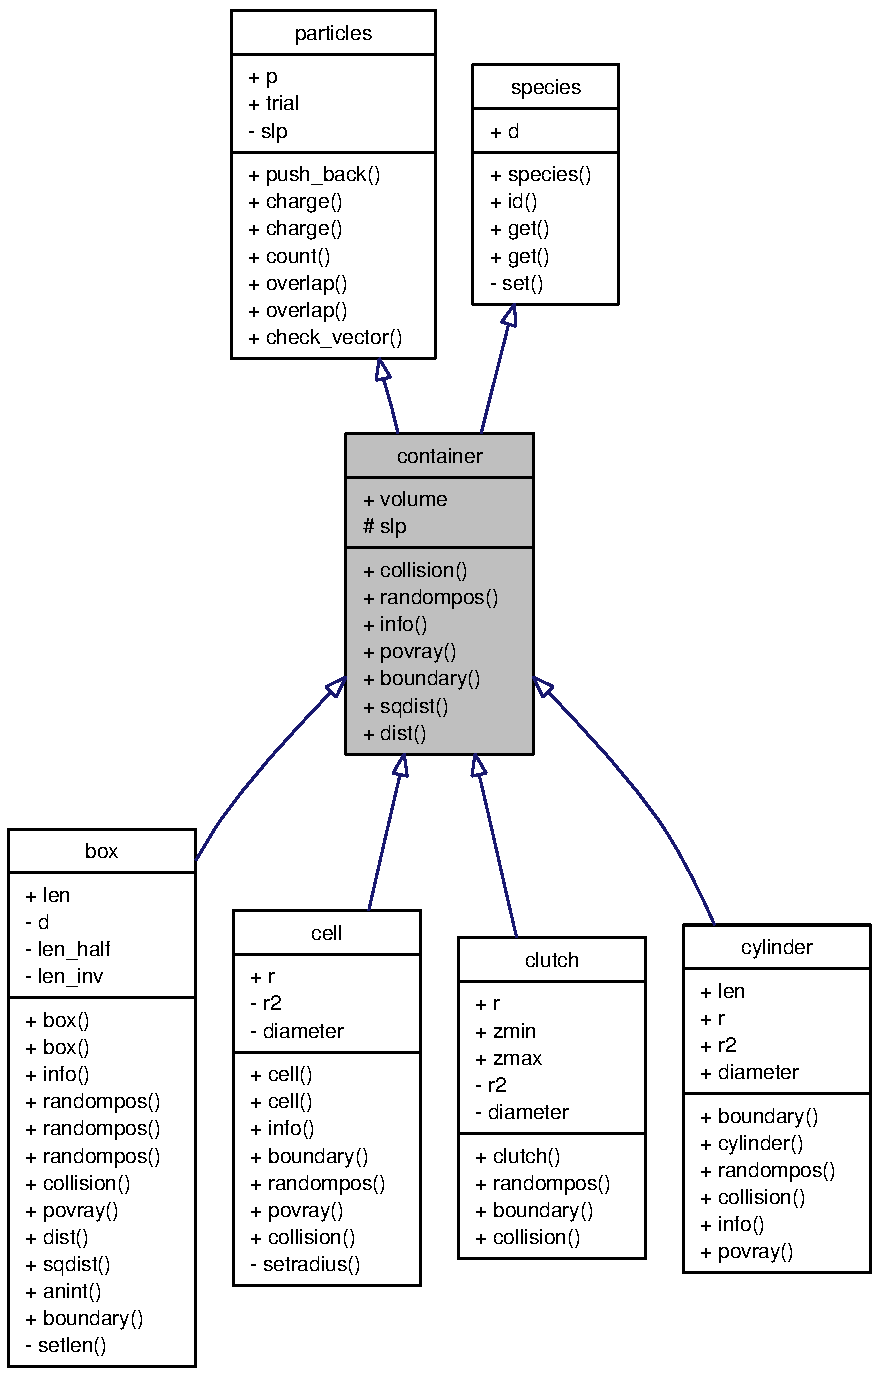
\includegraphics[width=6cm]{pics/container}
      \caption{fig}
      \label{fig:container}
	\end{figure}

  \subsection*{Figure 2 - Source code example}
      Example of a Monte Carlo simulation program to calculate protein
      ionization states in an aqueous salt solutions using explicit ions as well as
      a slightly coarse grained protein model.
      \begin{figure}[ht]\center
      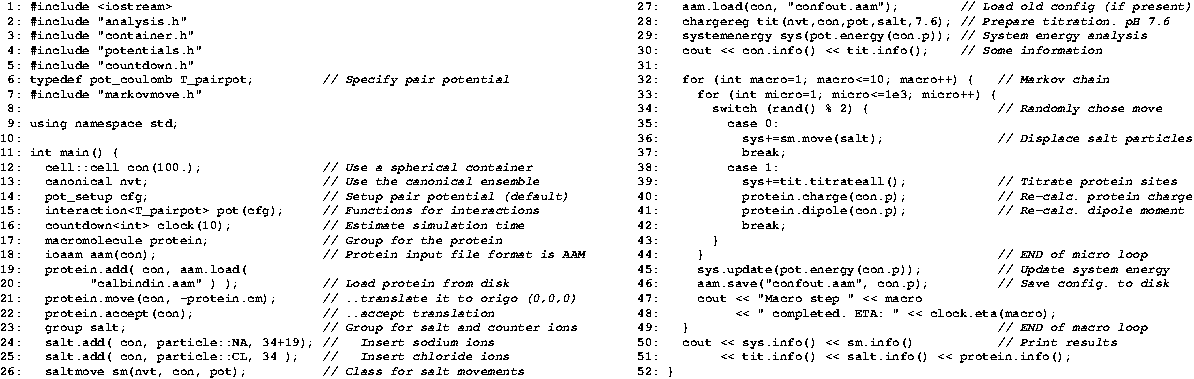
\includegraphics[width=16cm]{pics/source}
      \end{figure}
      
  \subsection*{Figure 3 - Povray output}
     Snapshot from a simulation of a single protein in a salt solution.
     \begin{figure}[ht]\center
      \includegraphics[width=6cm]{pics/snapshot}
      \end{figure}

\begin{comment}
%%%%%%%%%%%%%%%%%%%%%%%%%%%%%%%%%%%
%%                               %%
%% Tables                        %%
%%                               %%
%%%%%%%%%%%%%%%%%%%%%%%%%%%%%%%%%%%

%% Use of \listoftables is discouraged.
%%
\section*{Tables}
  \subsection*{Table 1 - Sample table title}
    Here is an example of a \emph{small} table in \LaTeX\ using  
    \verb|\tabular{...}|. This is where the description of the table 
    should go. \par \mbox{}
    \par
    \mbox{
      \begin{tabular}{|c|c|c|}
        \hline \multicolumn{3}{|c|}{My Table}\\ \hline
        A1 & B2  & C3 \\ \hline
        A2 & ... & .. \\ \hline
        A3 & ..  & .  \\ \hline
      \end{tabular}
      }
  \subsection*{Table 2 - Sample table title}
    Large tables are attached as separate files but should
    still be described here.



%%%%%%%%%%%%%%%%%%%%%%%%%%%%%%%%%%%
%%                               %%
%% Additional Files              %%
%%                               %%
%%%%%%%%%%%%%%%%%%%%%%%%%%%%%%%%%%%

\section*{Additional Files}
  \subsection*{Additional file 1 --- Sample additional file title}
    Additional file descriptions text (including details of how to
    view the file, if it is in a non-standard format or the file extension).  This might
    refer to a multi-page table or a figure.

  \subsection*{Additional file 2 --- Sample additional file title}
    Additional file descriptions text.
\end{comment}

\end{bmcformat}
\end{document}







